\documentclass{article}
\usepackage{geometry}
\usepackage{flafter}
\usepackage{float}
\geometry{letterpaper, portrait, margin=1in}

\usepackage{hyperref}
\hypersetup{
    colorlinks=true,
    linkcolor=black,
    filecolor=magenta,
    urlcolor=blue,
}

\usepackage{graphicx}
\graphicspath{ {images/} }

\usepackage{tcolorbox}
\usepackage{textcomp}
\usepackage{gensymb}
\usepackage{indentfirst}

\newcommand{\ans}{$\rule{1.5cm}{0.15mm}$}

\title{RoboJackets Electrical Training Week 3 Lab Guide}
\author{Eugene Min and Andrew Rocco}
\date{\today\\v1.0}

\begin{document}
\maketitle{}
\setcounter{tocdepth}{2}
\tableofcontents
\pagebreak

%Everything below is for you to edit. Code above sets up the general formatting for the document

\section{Background}
This week's lecture topic was on designing schematics with Eagle. RoboJackets teams will mainly be using Eagle to design printed circuit boards (PCBs) for their robots. For this reason, it is important to feel comfortable using this software and learn about the many different features Eagle offers for PCB design.

In this lab, you will be given a partially built schematic for a PCB. Your objective is to complete this PCB using the parts list given below. You will have to use the various RoboJackets libraries to add these parts to the schematic. 


\section{Objective}
\subsection{Task 1}
\begin{itemize}
    \item Find the desired parts in the RoboJackets libraries. This step will be required for the the parts of the lab that ask you to insert parts into the schematic
\end{itemize}
\subsection{Task 2}
\begin{itemize}
    \item Place parts from the parts list into their respective places in the schematic.
\end{itemize}
\subsection{Task 3}
\begin{itemize}
    \item Create connections between different components in the schematic where they are needed
\end{itemize}
\section{Materials}
\begin{itemize}
	\item EAGLE CAD
	\item \texttt{eagle-libraries} correctly configured
	\item Schematic Template
\end{itemize}

\section{Relevant Information}
\subsection{Adding libraries to Eagle}
To add libraries to your Eagle directory, first download the libraries. Then, go to the Eagle Control Panel and select the “Options” tab. Then select “Directories…”. At this point, you can browse your computer and find where the libraries are located. You should have configured your library setup in Week 2, following the instructions on the README in the \texttt{eagle-libraries} repository. 
\begin{figure}[ht]
	\center
	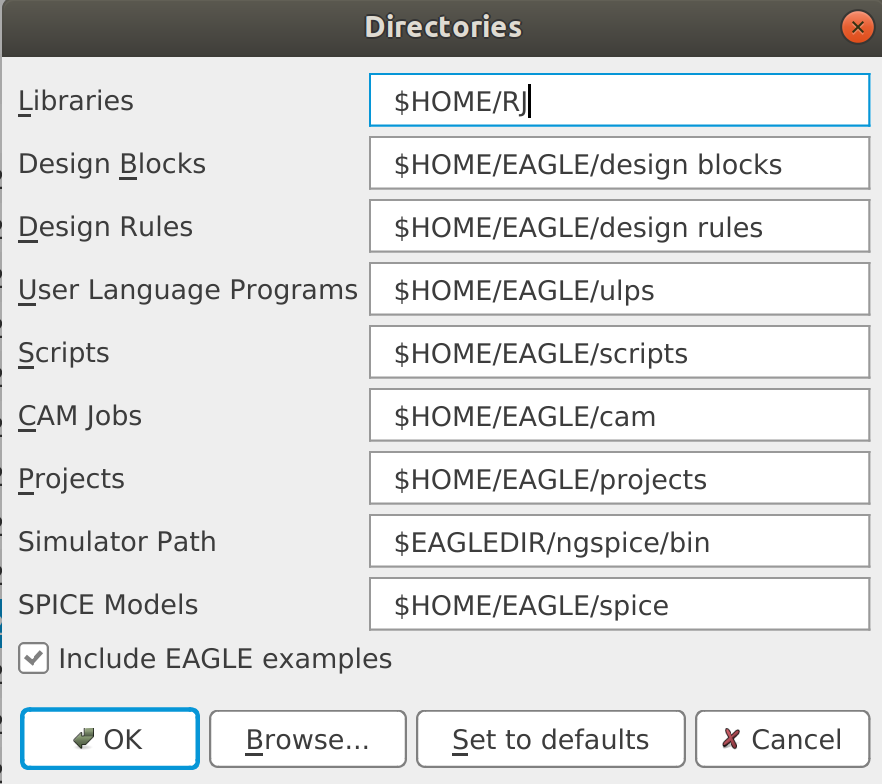
\includegraphics[width=0.3\textwidth, keepaspectratio]{images/directories.png}
	\caption{Directories menu}
	\label{fig:directories}
\end{figure}
\subsection{Putting libraries in use}
To use these libraries, you will have to put them in use in the schematic. In the schematic view, go to the “Library” tab at the top then click on “Open library manager”. Go to “Available” then highlight the libraries you want to use, which are the RoboJackets libraries in this case. 
\begin{figure}[ht]
	\center
	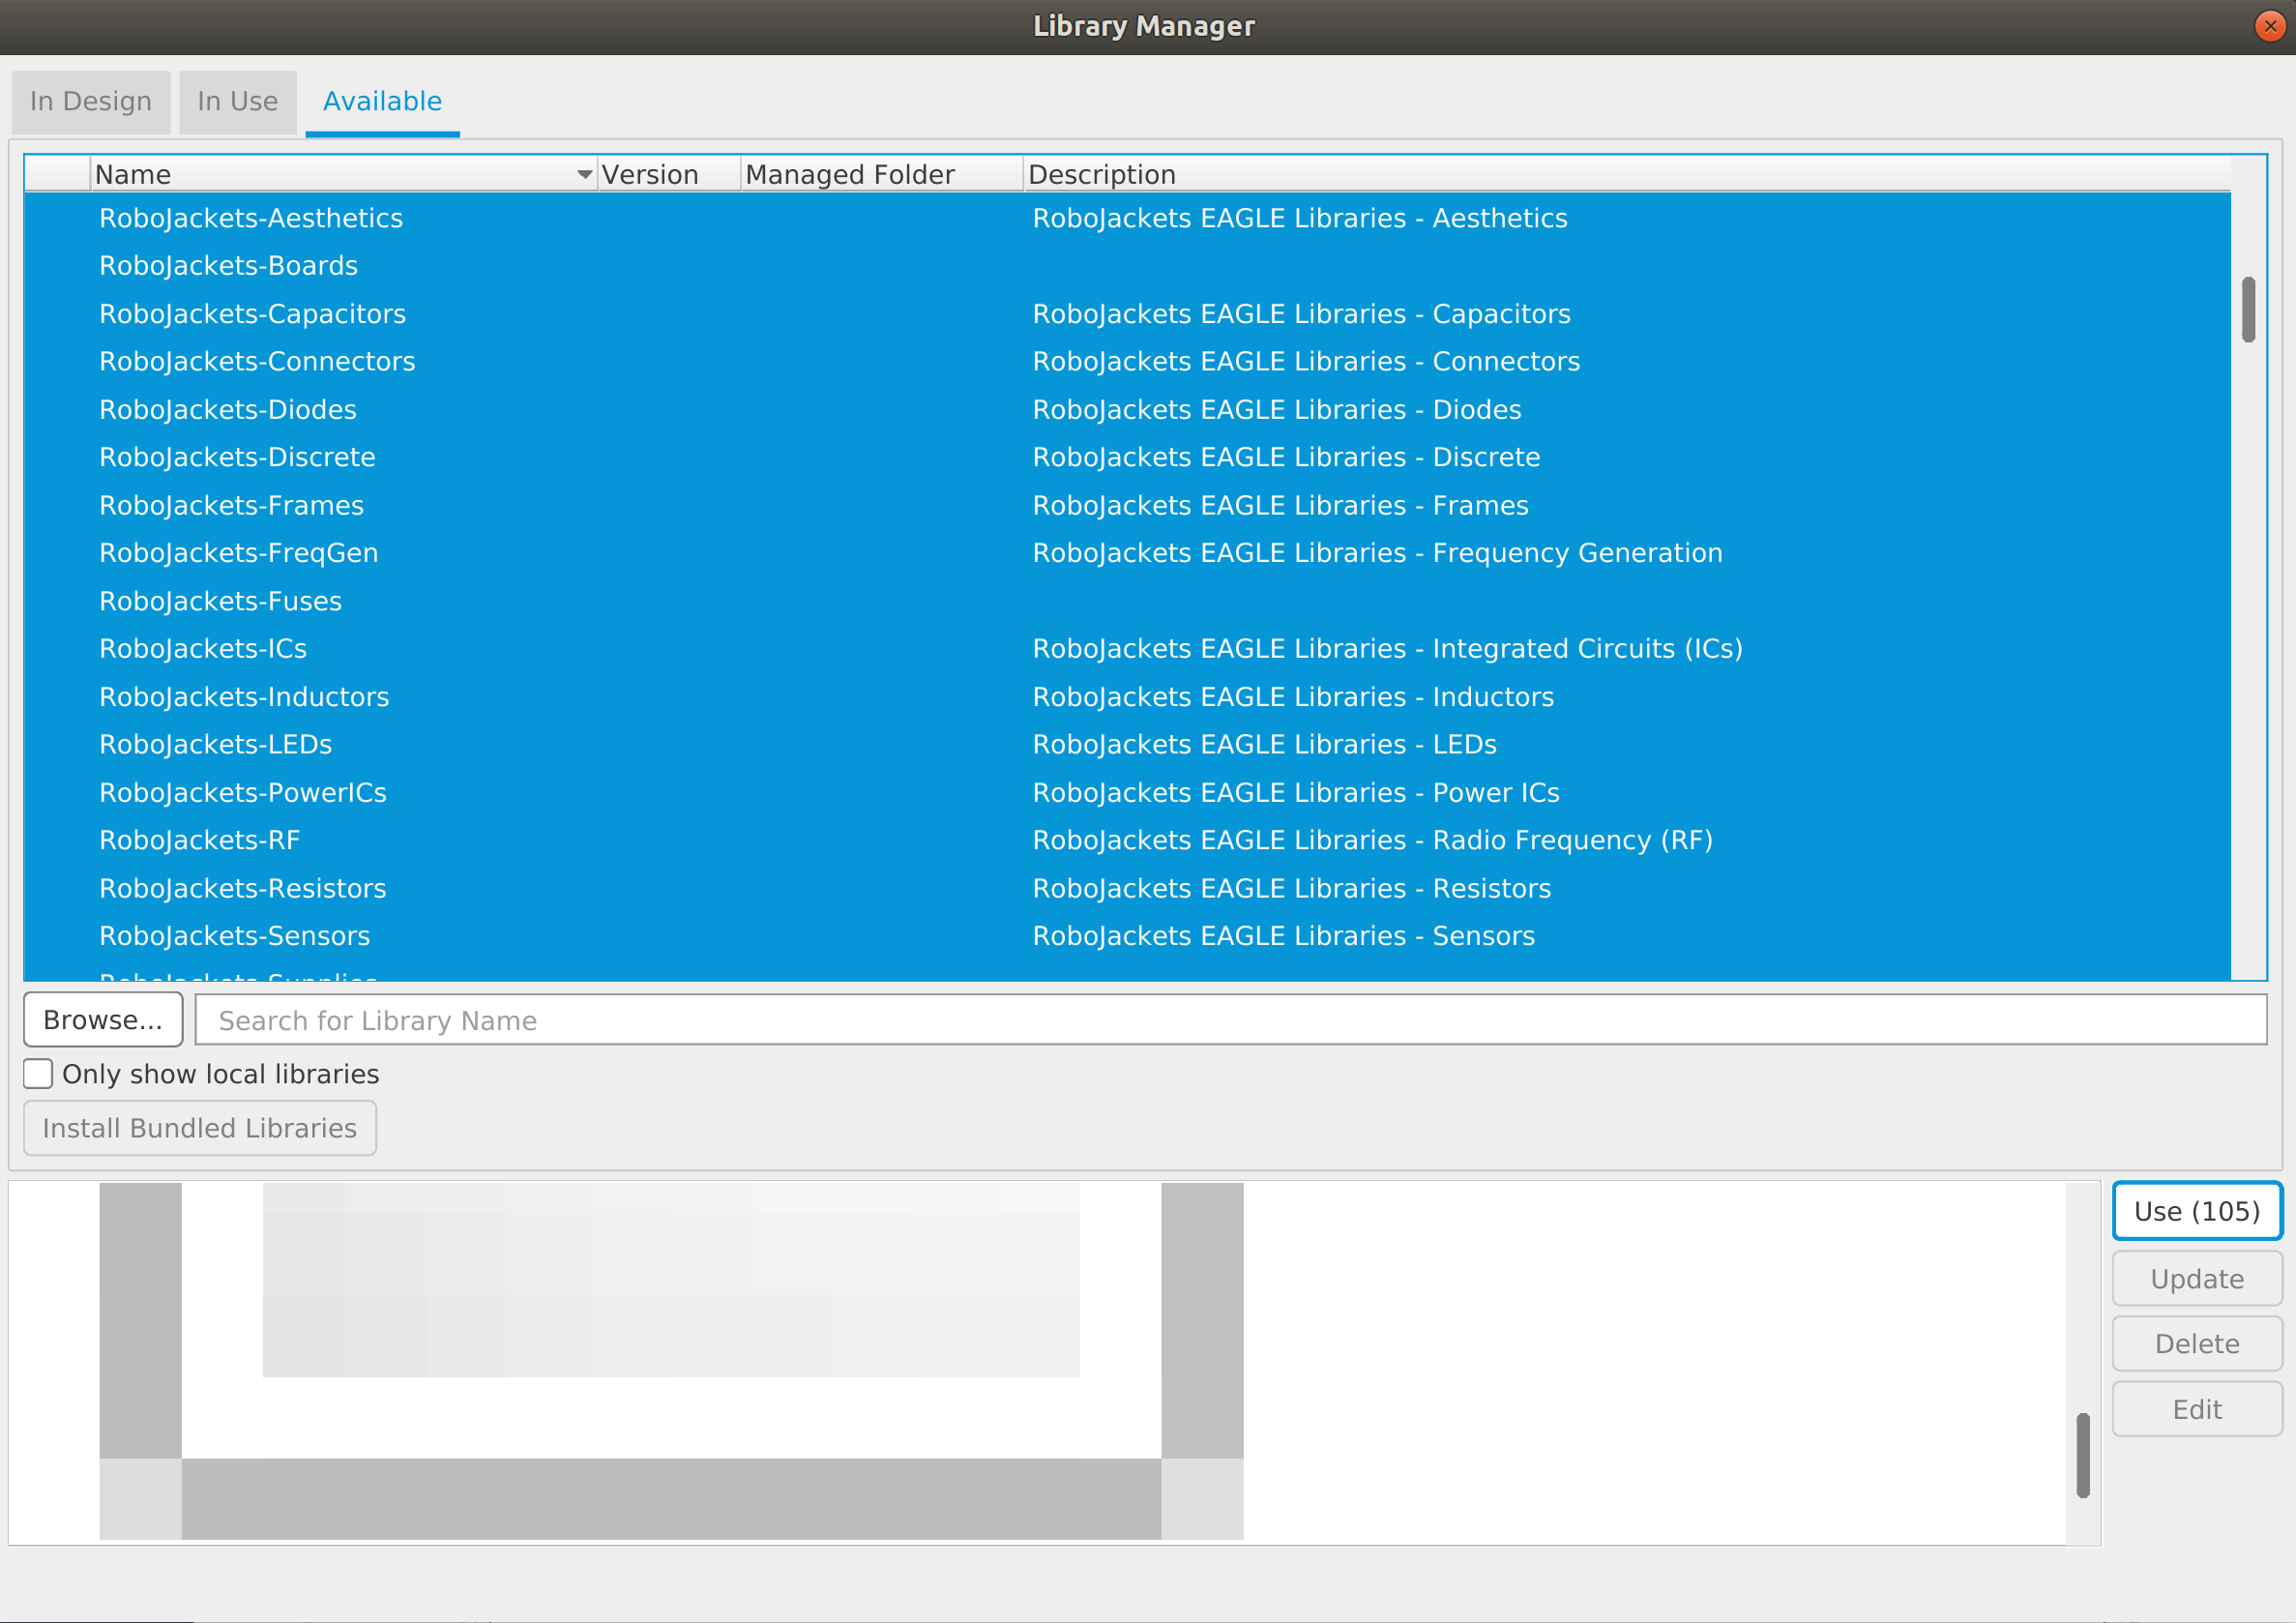
\includegraphics[width=0.6\textwidth, keepaspectratio]{images/manager.png}
	\caption{Including RoboJackets Libraries}
	\label{fig:addlib}
\end{figure}
\subsection{Adding parts to your schematic}
With the libraries available to use, you can select the “Add Part” button located in the left menu in the schematic and search for the desired part. Use the “*” character at the front and end of the search term for a wider search.
\begin{figure}[ht]
	\center
	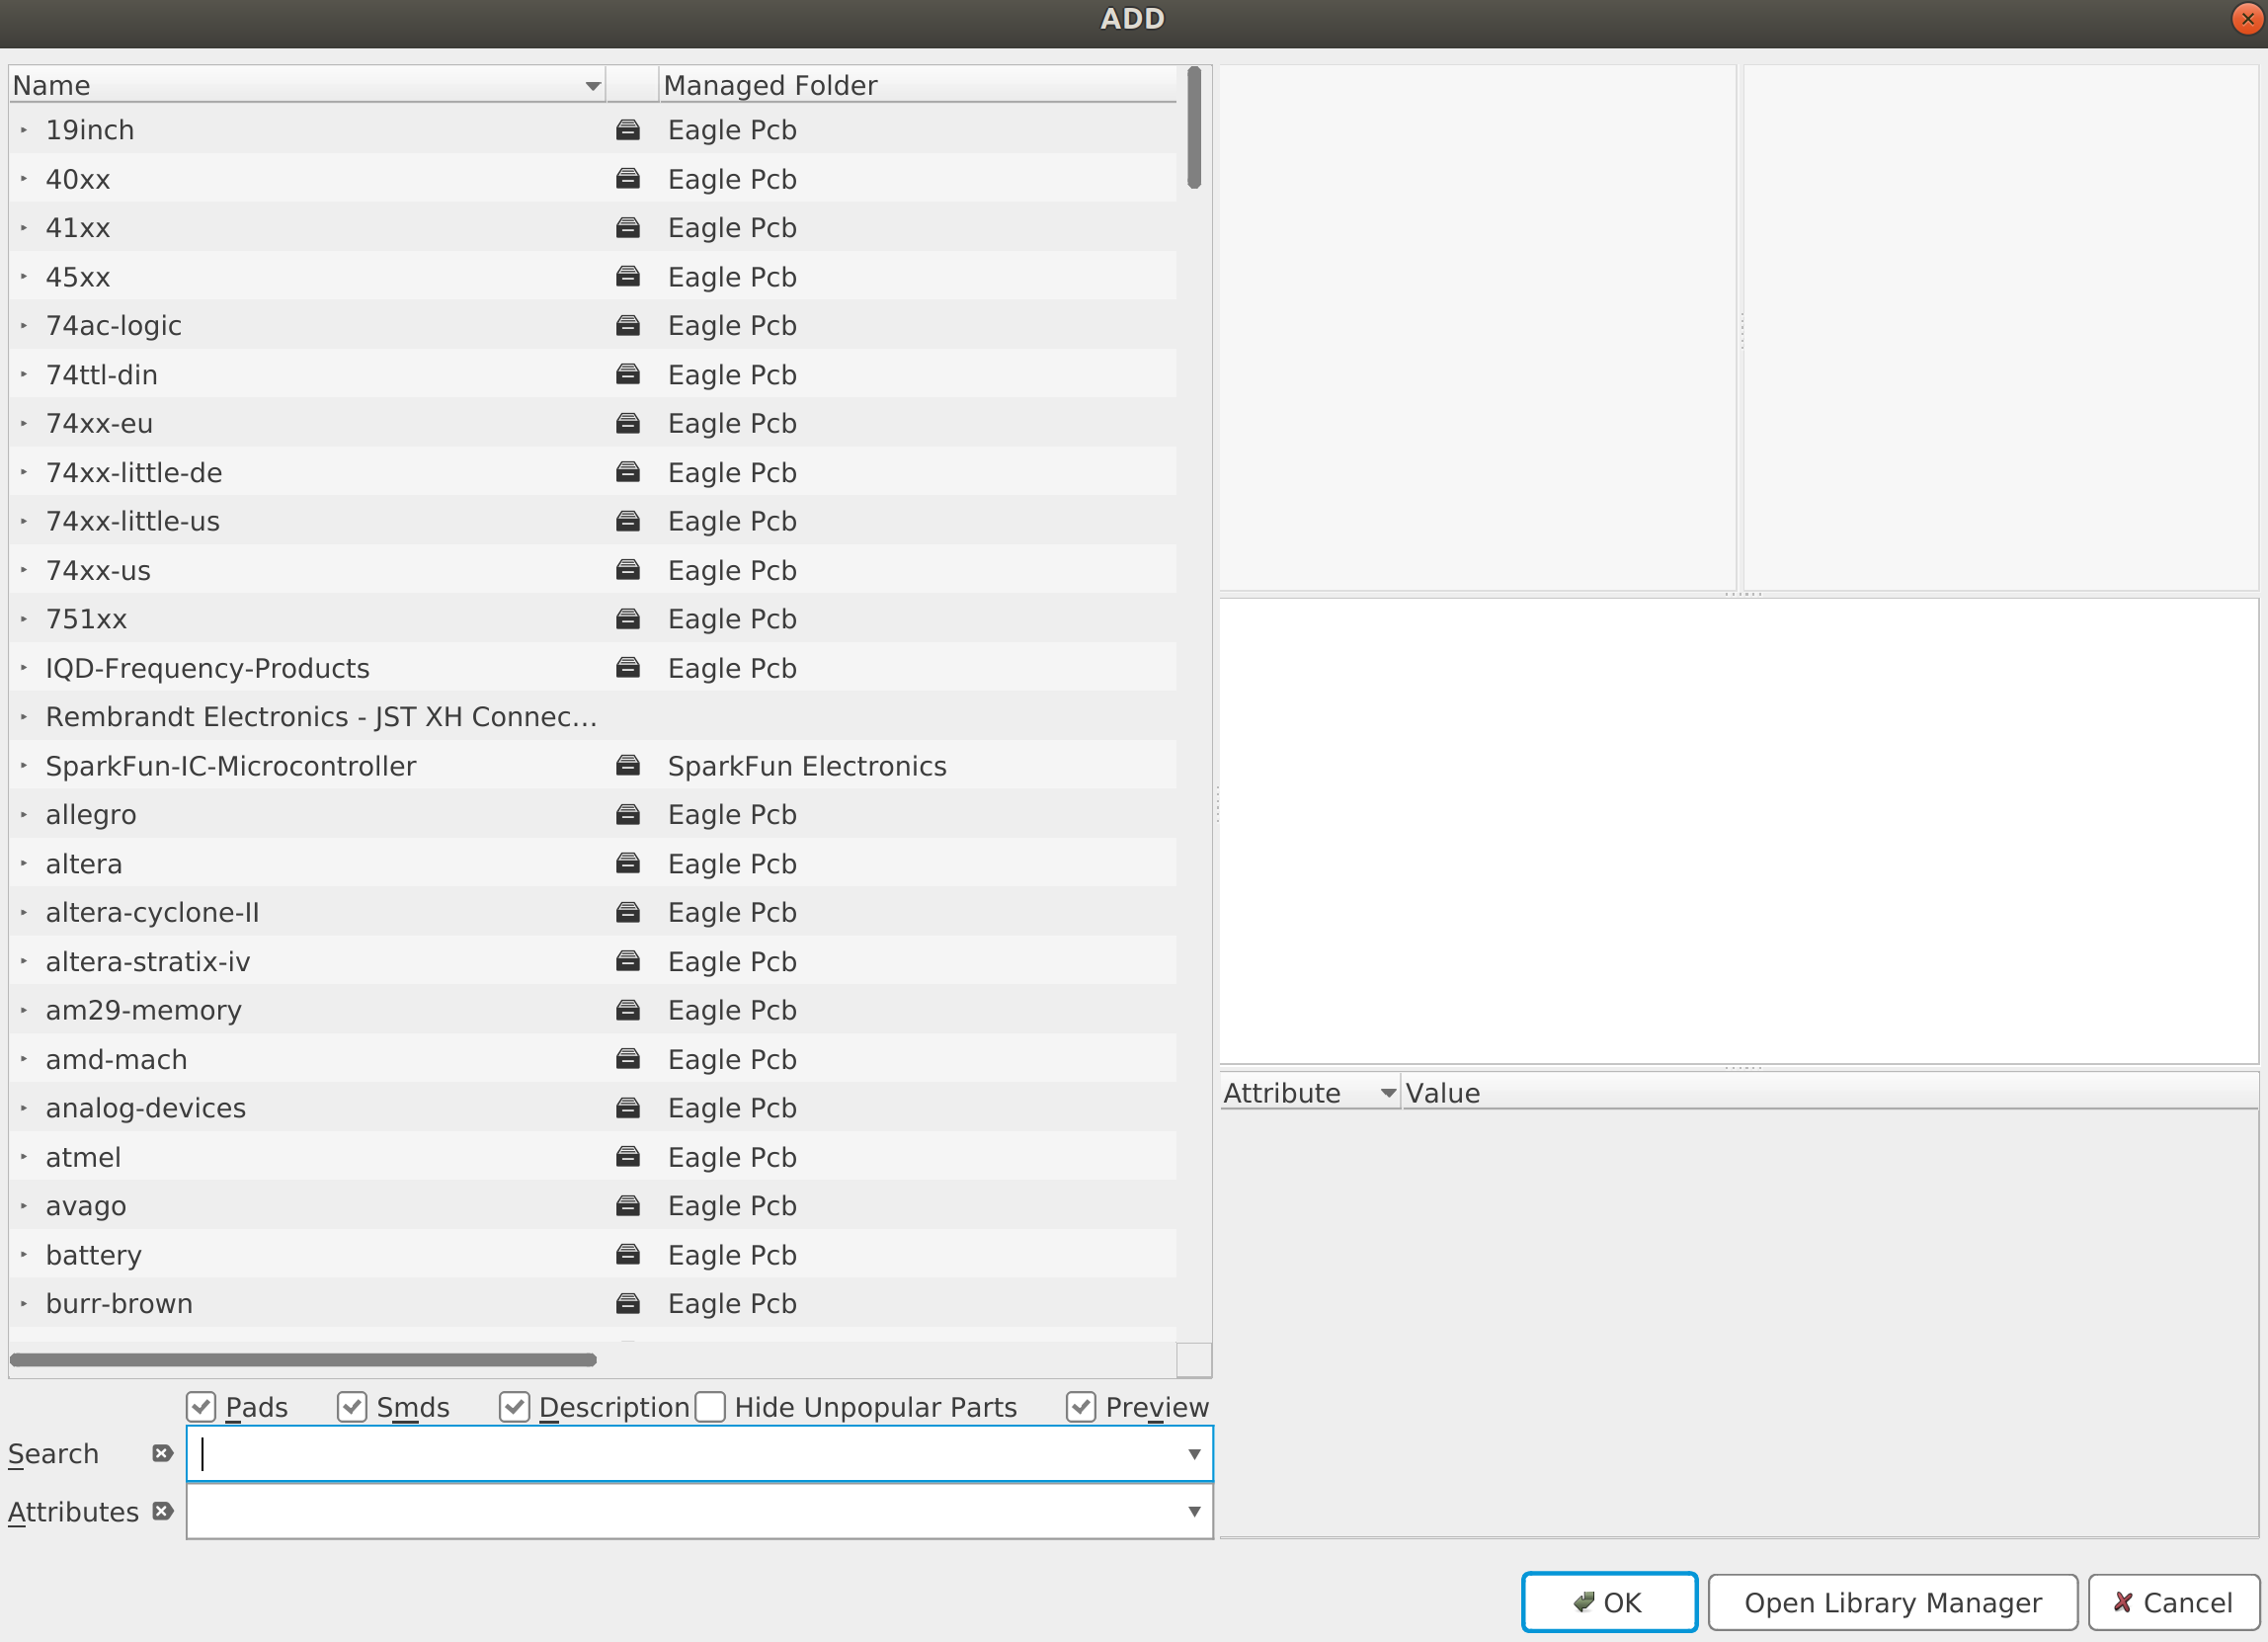
\includegraphics[width=0.6\textwidth, keepaspectratio]{images/addpart.png}
	\caption{Add Part Menu}
	\label{fig:addpart}
\end{figure}
\subsection{Making connections}
Once placing a part in the schematic, you can use the “Net” button in the left menu to connect two parts. If there are connections that need to be made far away from each other, you can use the “Label” button in the left menu to do this. Create a short net from one part and  place a label at the end of it. Do the same where you want to place the other end of the connection. TO get the triangular labels rather than the text labels, turn "xref on" using a button in the top menu and shown in the picture below. 

\begin{figure}[H]
  \centering
  \begin{minipage}[b]{0.3\textwidth}
    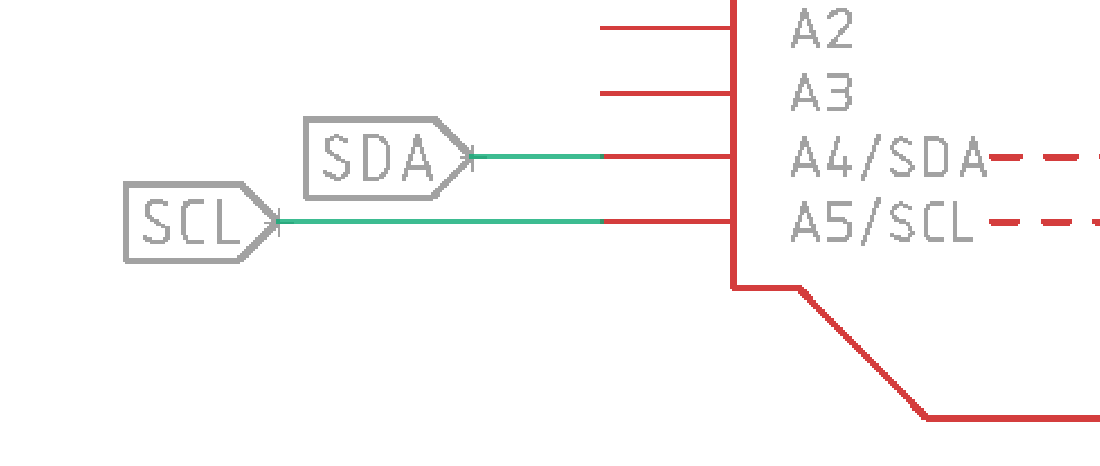
\includegraphics[width=\textwidth]{xref.png}
    \caption{Adding Labels}
  \end{minipage}
  \hfill
  \begin{minipage}[b]{0.3\textwidth}
    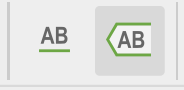
\includegraphics[width=\textwidth]{xrefsymbol.png}
    \caption{Turning Xref setting on}
  \end{minipage}
\end{figure}

\section{Guided Lab}
\subsection{Add an 0603 pull-down resistor to the SW1 Buttons circuit}
\begin{itemize}
    \item Select “Add part” and search for an 0603 resistor in the \texttt{rcl} library. This should be in the R-US\_ folder and called R-US\_R0603
    \item  Place the resistor in the correct place in the circuit. Orientation of resistors is not important.
    \item Create connections on both sides of the resistor.
    \item Give the resistor the value “10K” (10,000 ohms). This can be done by clicking the "Value" button in the left menu and clicking the part or by typing \texttt{value} in the EAGLE command line. 
\end{itemize}
Purpose: This resistor is needed in the circuit to ensure that when switch “SW1” is open, the "SW1\_INT" signal is not floating but 0V.
\begin{figure}[ht]
	\center
	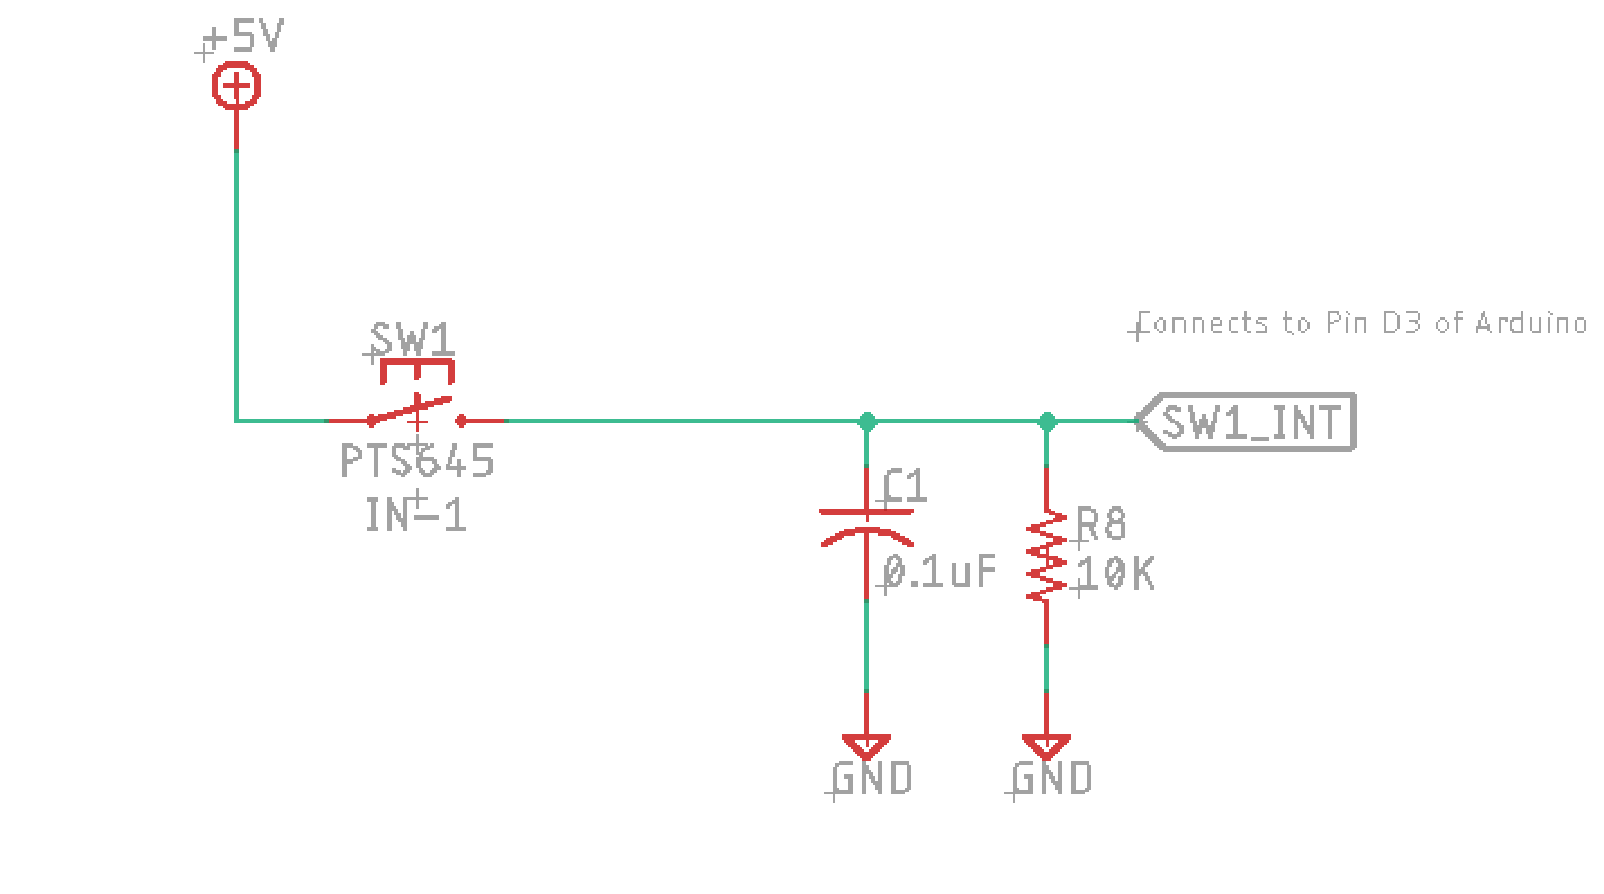
\includegraphics[width=0.5\textwidth, keepaspectratio]{images/5.1.png}
	\caption{Adding resistor}
	\label{fig:5.1}
\end{figure}
\subsection{Add a PTS645 button to the SW2 Buttons circuit}
\begin{itemize}
    \item  Select “Add part” and search for a PTS645 button in the RoboJackets - Switches library. This part is a normally open pushbutton. When pushed, the circuit is closed, otherwise it is open.
    \item Place the button in the correct place in the circuit.
    \item Create connections on both sides of the button as shown in the picture.
\end{itemize}
\begin{figure}[ht]
	\center
	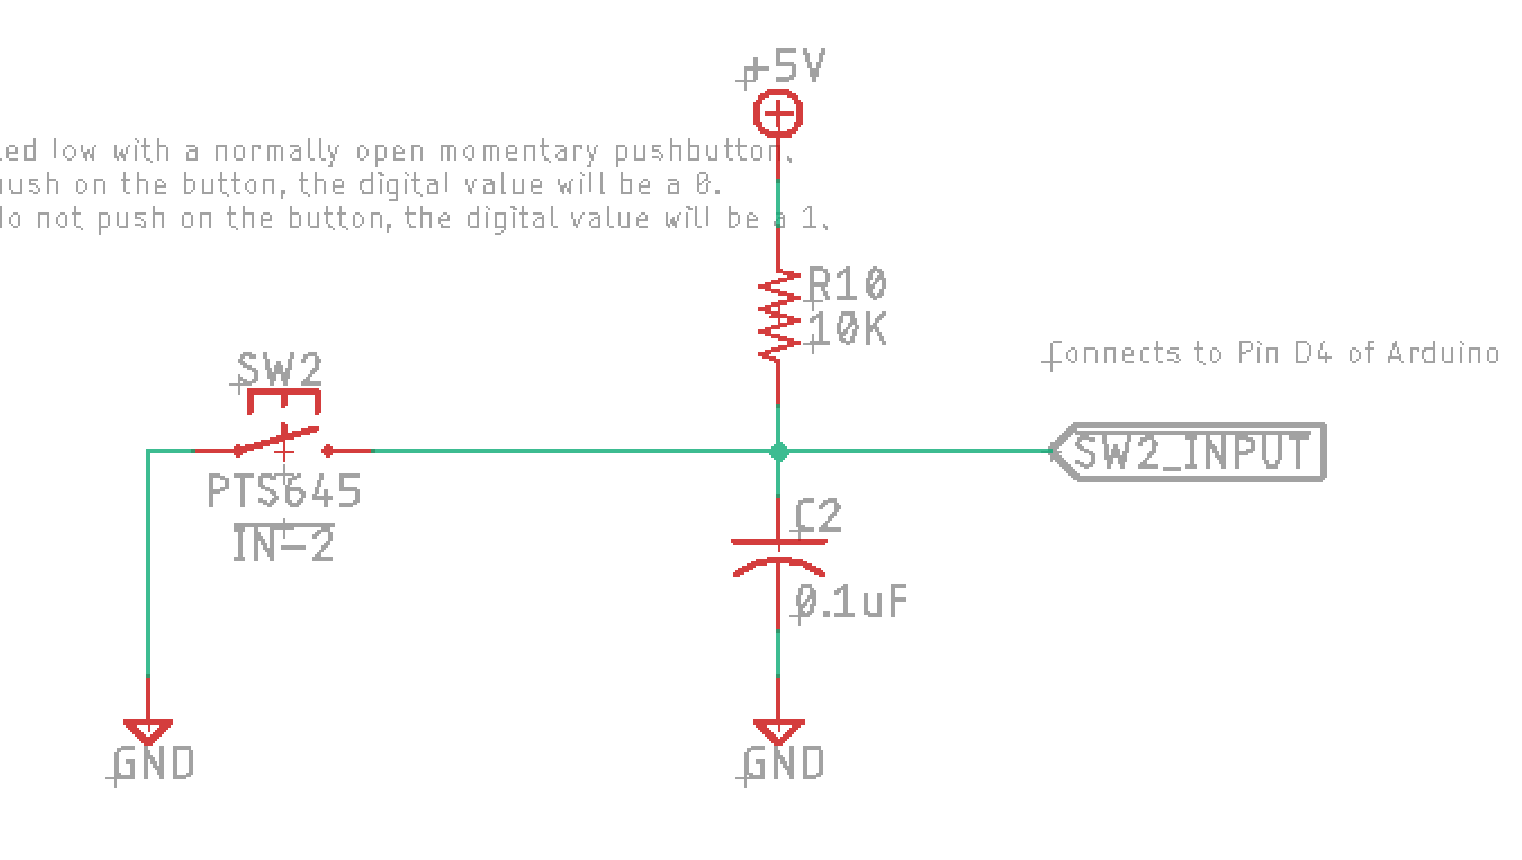
\includegraphics[width=0.5\textwidth, keepaspectratio]{images/5.2.png}
	\caption{Adding switch}
	\label{fig:5.2}
\end{figure}
\subsection{Add a 5V supply for the pull-up resistor in the “!RESET” circuit}
\begin{itemize}
    \item Select “Add part” and search for a +5V supply in the RoboJackets-Supplies library. This will signify a connection to the 5V source on the board to this point of the circuit.
    \item Place the part in the correct place in the circuit.
    \item Create a connection from the +5V supply to resistor R13.
\end{itemize}
\begin{figure}[ht]
	\center
	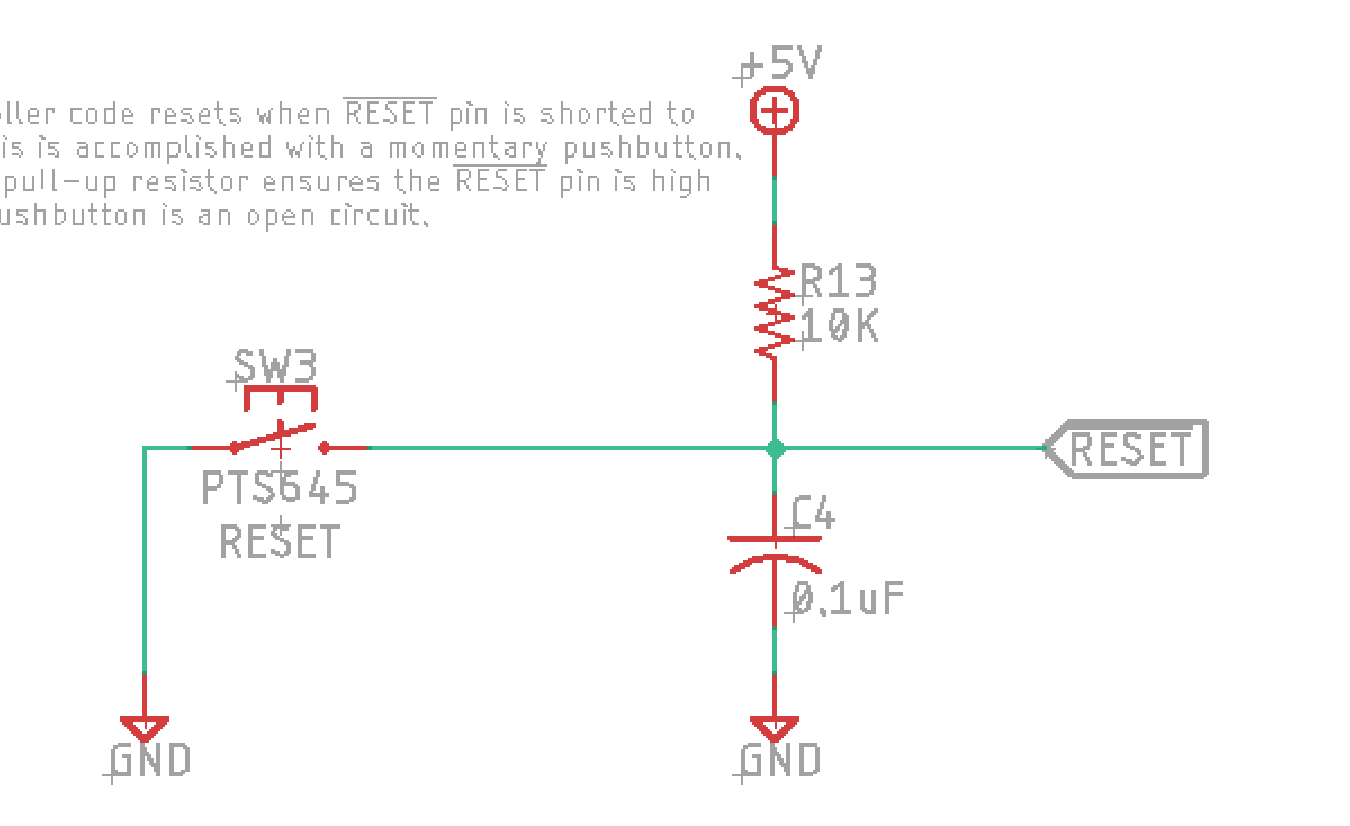
\includegraphics[width=0.5\textwidth, keepaspectratio]{images/5.3.png}
	\caption{Adding 5V supply}
	\label{fig:5.3}
\end{figure}
\subsection{Create a connection for the signal “D2\_CTRL” using labels}
\begin{itemize}
    \item Create a net from pin D10 on the Arduino Uno Microcontroller to a label. This will signify a connection to the +5V source on the board to this point of the circuit.
    \item  Name the label “D2\_CTRL”. The name you give a label corresponds to the name of its signal. In this case, the D10 pin is controlling the D2 led, so naming the signal “D2\_CTRL” is a good way to signify what that signal controls.
    \begin{figure}[ht]
	\center
	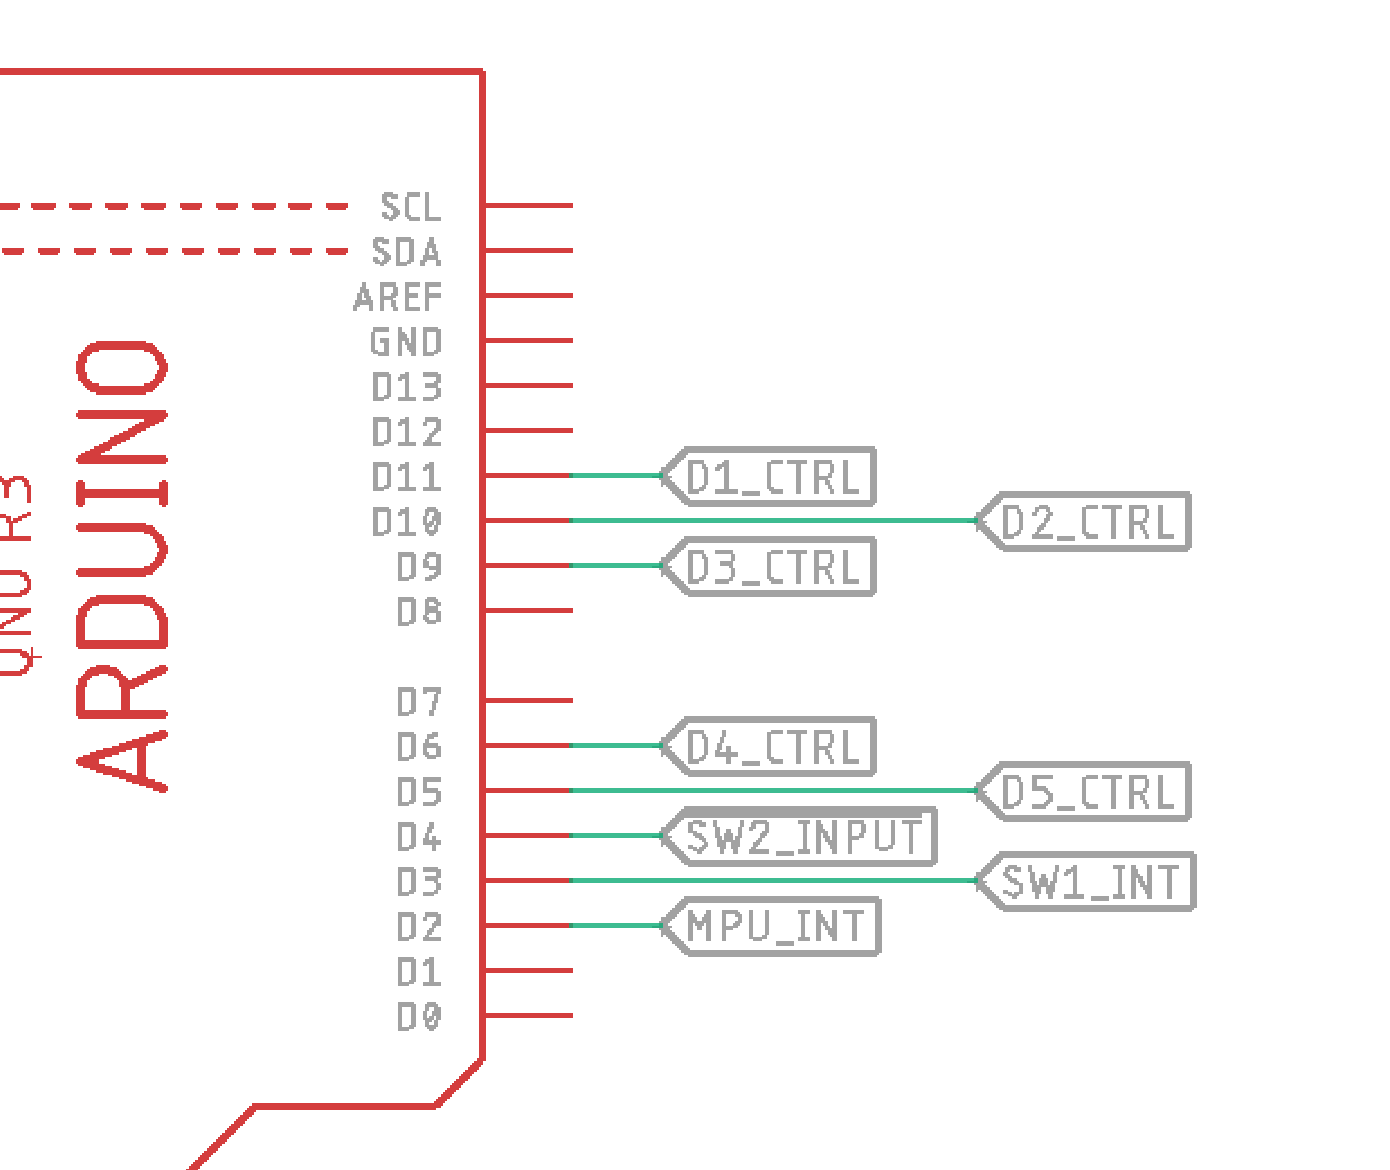
\includegraphics[width=0.3\textwidth, keepaspectratio]{images/5.4.1.png}
	\caption{Adding D2\_CTRL label on D10}
	\label{fig:5.4.1}
\end{figure}
    \item Create another label and net that connect to the second resistor from the top in the “LEDs” section.  Give this label the same name as the signal from D10.
    \begin{figure}[ht]
	\center
	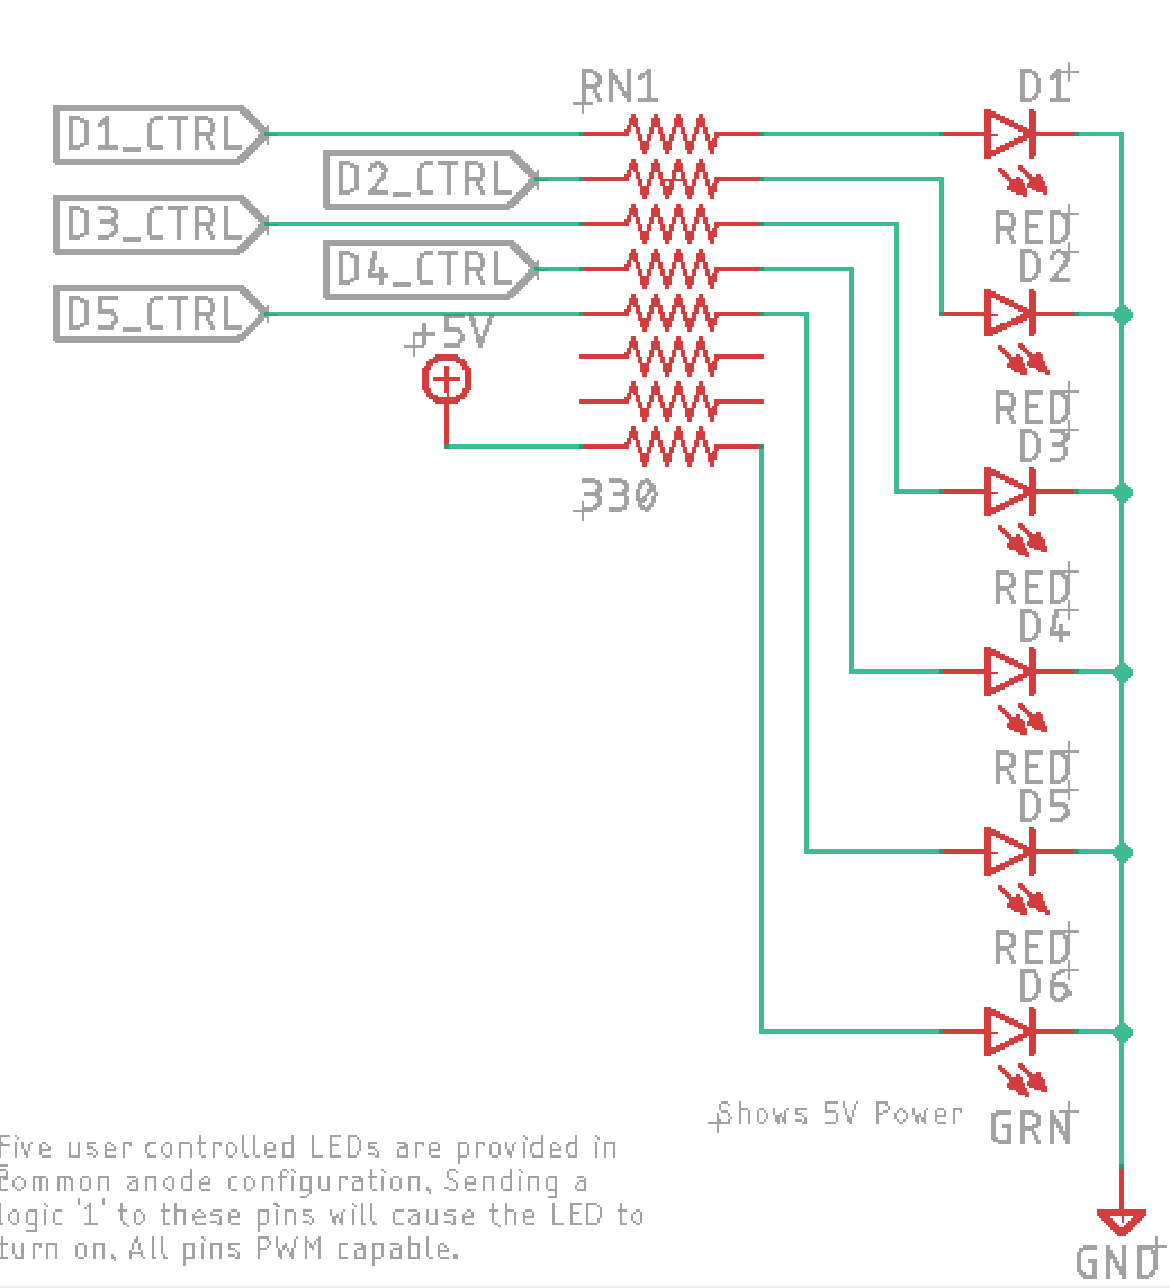
\includegraphics[width=0.3\textwidth, keepaspectratio]{images/5.4.2.png}
	\caption{Adding D2\_CTRL label on second LED}
	\label{fig:5.4.2}
    \end{figure}
    \item You should then be asked if you want to create a connection. Select “Yes”.
\end{itemize}
Purpose: This method of connecting different parts that are far apart will make the schematic cleaner and easier to read. But, a physical connection will need to be made when you are designing the board itself. To get a better idea of this, press the schematic to board button (located in the upper left) and create the board. Here, you will see all of the physical connections that need to be made. Connections denoted using labels in the schematic need to be physically connected here, as shown by the thin yellow lines. This will be the topic of next week’s training.
\begin{figure}[H]
	\center
	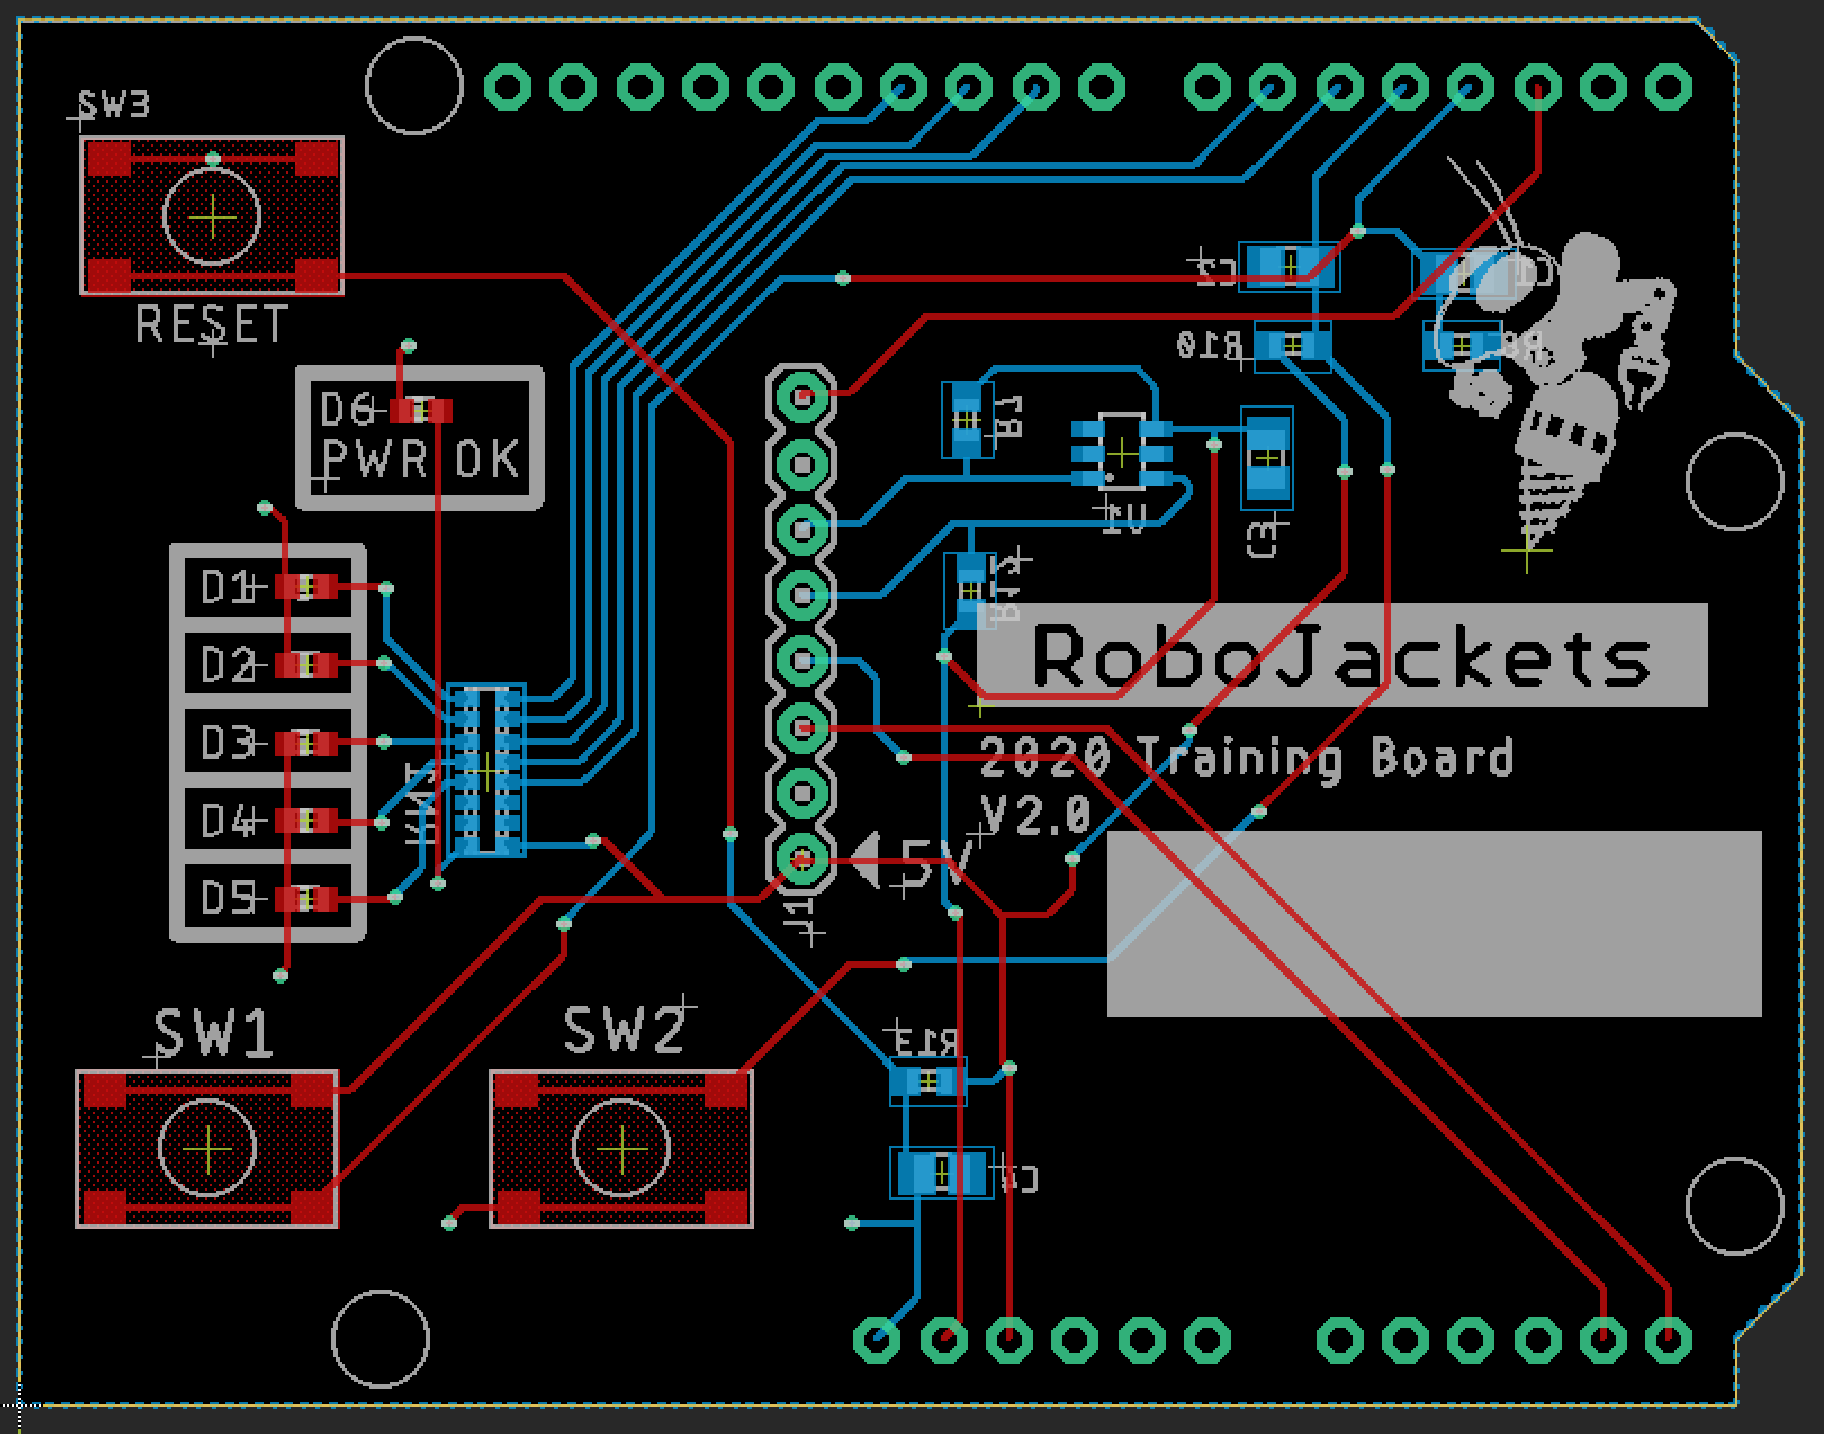
\includegraphics[width=0.4\textwidth, keepaspectratio]{images/board.png}
	\caption{Next week's lab involves routing the board this schematic creates! This is what the finished routing looks like.}
	\label{fig:board}
\end{figure}
\subsection{Use the pictures and parts list to design the circuit shown in the picture}
\begin{itemize}
    \item Parts List:
\begin{itemize}
    \item Sensor: TLE493DA2B6HTSA1 (in RoboJackets-ICs)
    \item Resistors: R0603 (in rcl)
    \item Capacitor: C0805 (in rcl)
    \item +3.3V (RoboJackets-Supplies)
    \item GND (RoboJackets-Supplies)
\end{itemize}
    \item Connect the XDA signal to pin 5 on the axis sensor.
    \item Connect the XCL signal to pin 6 on the axis sensor.
\end{itemize}
\begin{figure}[H]
	\center
	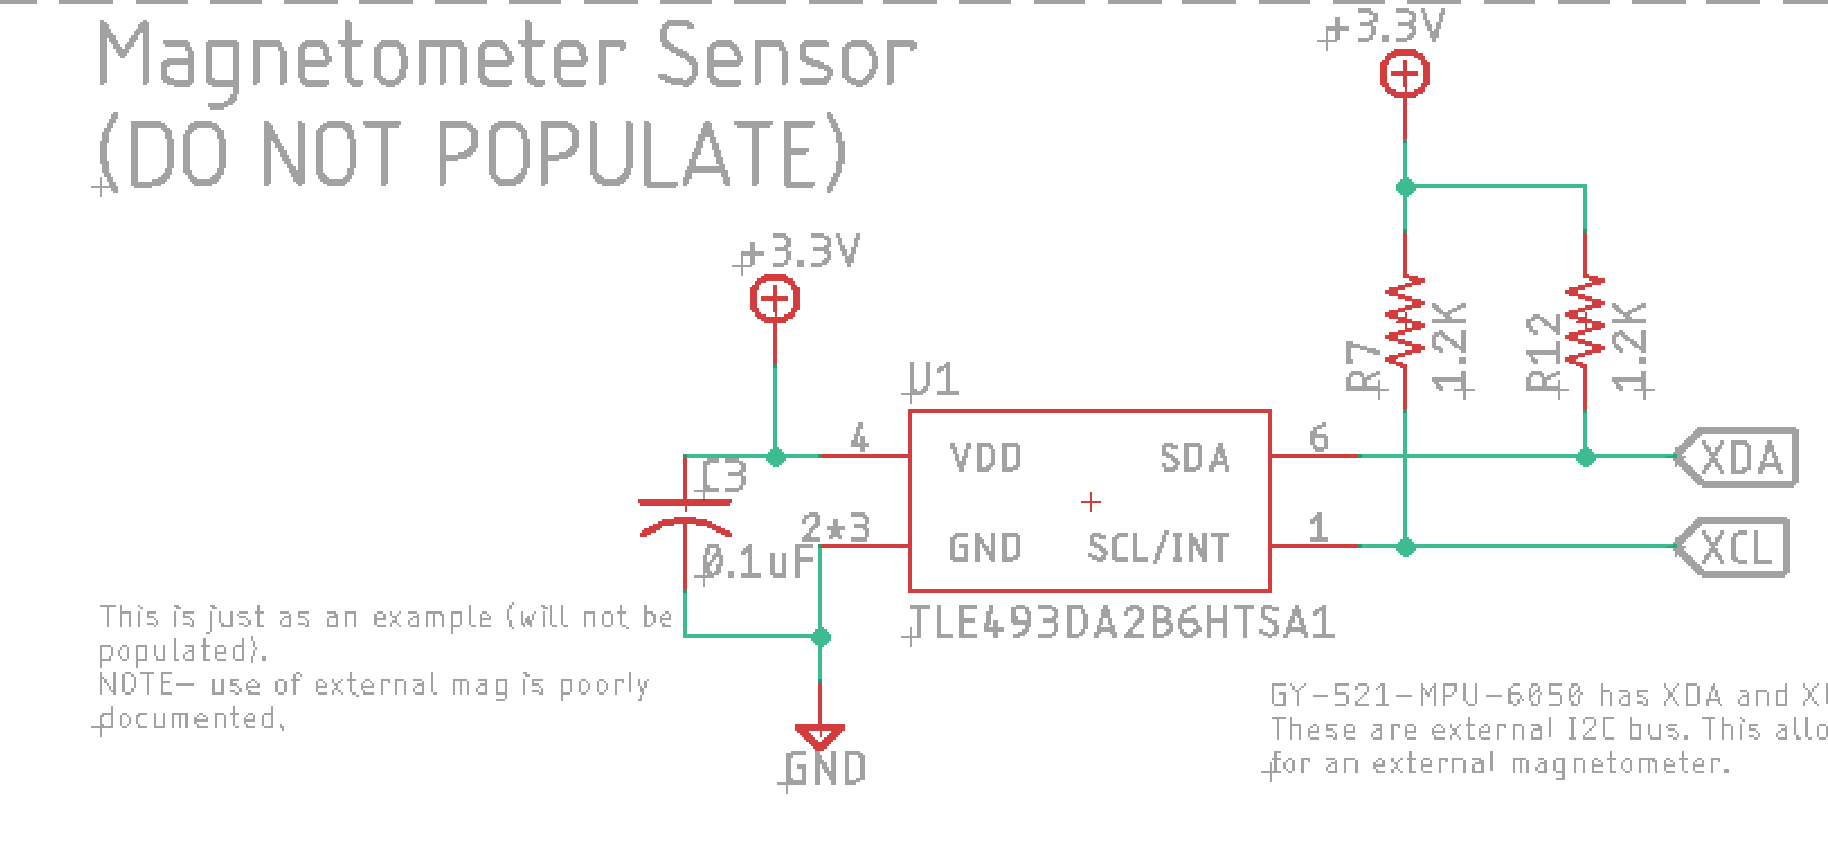
\includegraphics[width=0.8\textwidth, keepaspectratio]{images/5.5.png}
	\caption{Adding magnetometer circuit}
	\label{fig:5.5}
\end{figure}

\section{Troubleshooting}
\begin{itemize}
    \item \href{https://github.com/RoboJackets/electrical-training/blob/master/references/eagle_cheat_sheet/eagle_cheat_sheet.pdf}{EAGLE Cheat Sheet}: Use this for instructions using Eagle and its functions.
    \item \href{https://www.youtube.com/watch?v=gEWAhHHDmQk}{EAGLE Schematics Video}: Reference this video for a walkthrough of creating a schematic.
    \item \href{https://wiki.robojackets.org/EAGLE_Style_Guide}{RoboJackets EAGLE Style Guide}: This document is a set of guidelines Robojackets uses when creating parts and schematics.
    \item \href{https://github.com/RoboJackets/eagle-libraries} {EAGLE Setup Guide}: If you need help installing Eagle, reference this document.
\end{itemize}

\end{document}